% Options for packages loaded elsewhere
\PassOptionsToPackage{unicode}{hyperref}
\PassOptionsToPackage{hyphens}{url}
\PassOptionsToPackage{dvipsnames,svgnames,x11names}{xcolor}
%
\documentclass[
  a4paper,
  DIV=11,
  numbers=noendperiod]{scrartcl}

\usepackage{amsmath,amssymb}
\usepackage{iftex}
\ifPDFTeX
  \usepackage[T1]{fontenc}
  \usepackage[utf8]{inputenc}
  \usepackage{textcomp} % provide euro and other symbols
\else % if luatex or xetex
  \usepackage{unicode-math}
  \defaultfontfeatures{Scale=MatchLowercase}
  \defaultfontfeatures[\rmfamily]{Ligatures=TeX,Scale=1}
\fi
\usepackage{lmodern}
\ifPDFTeX\else  
    % xetex/luatex font selection
\fi
% Use upquote if available, for straight quotes in verbatim environments
\IfFileExists{upquote.sty}{\usepackage{upquote}}{}
\IfFileExists{microtype.sty}{% use microtype if available
  \usepackage[]{microtype}
  \UseMicrotypeSet[protrusion]{basicmath} % disable protrusion for tt fonts
}{}
\makeatletter
\@ifundefined{KOMAClassName}{% if non-KOMA class
  \IfFileExists{parskip.sty}{%
    \usepackage{parskip}
  }{% else
    \setlength{\parindent}{0pt}
    \setlength{\parskip}{6pt plus 2pt minus 1pt}}
}{% if KOMA class
  \KOMAoptions{parskip=half}}
\makeatother
\usepackage{xcolor}
\usepackage[top=20mm,bottom=20mm,left=20mm,right=20mm,heightrounded]{geometry}
\setlength{\emergencystretch}{3em} % prevent overfull lines
\setcounter{secnumdepth}{-\maxdimen} % remove section numbering
% Make \paragraph and \subparagraph free-standing
\ifx\paragraph\undefined\else
  \let\oldparagraph\paragraph
  \renewcommand{\paragraph}[1]{\oldparagraph{#1}\mbox{}}
\fi
\ifx\subparagraph\undefined\else
  \let\oldsubparagraph\subparagraph
  \renewcommand{\subparagraph}[1]{\oldsubparagraph{#1}\mbox{}}
\fi

\usepackage{color}
\usepackage{fancyvrb}
\newcommand{\VerbBar}{|}
\newcommand{\VERB}{\Verb[commandchars=\\\{\}]}
\DefineVerbatimEnvironment{Highlighting}{Verbatim}{commandchars=\\\{\}}
% Add ',fontsize=\small' for more characters per line
\usepackage{framed}
\definecolor{shadecolor}{RGB}{241,243,245}
\newenvironment{Shaded}{\begin{snugshade}}{\end{snugshade}}
\newcommand{\AlertTok}[1]{\textcolor[rgb]{0.68,0.00,0.00}{#1}}
\newcommand{\AnnotationTok}[1]{\textcolor[rgb]{0.37,0.37,0.37}{#1}}
\newcommand{\AttributeTok}[1]{\textcolor[rgb]{0.40,0.45,0.13}{#1}}
\newcommand{\BaseNTok}[1]{\textcolor[rgb]{0.68,0.00,0.00}{#1}}
\newcommand{\BuiltInTok}[1]{\textcolor[rgb]{0.00,0.23,0.31}{#1}}
\newcommand{\CharTok}[1]{\textcolor[rgb]{0.13,0.47,0.30}{#1}}
\newcommand{\CommentTok}[1]{\textcolor[rgb]{0.37,0.37,0.37}{#1}}
\newcommand{\CommentVarTok}[1]{\textcolor[rgb]{0.37,0.37,0.37}{\textit{#1}}}
\newcommand{\ConstantTok}[1]{\textcolor[rgb]{0.56,0.35,0.01}{#1}}
\newcommand{\ControlFlowTok}[1]{\textcolor[rgb]{0.00,0.23,0.31}{#1}}
\newcommand{\DataTypeTok}[1]{\textcolor[rgb]{0.68,0.00,0.00}{#1}}
\newcommand{\DecValTok}[1]{\textcolor[rgb]{0.68,0.00,0.00}{#1}}
\newcommand{\DocumentationTok}[1]{\textcolor[rgb]{0.37,0.37,0.37}{\textit{#1}}}
\newcommand{\ErrorTok}[1]{\textcolor[rgb]{0.68,0.00,0.00}{#1}}
\newcommand{\ExtensionTok}[1]{\textcolor[rgb]{0.00,0.23,0.31}{#1}}
\newcommand{\FloatTok}[1]{\textcolor[rgb]{0.68,0.00,0.00}{#1}}
\newcommand{\FunctionTok}[1]{\textcolor[rgb]{0.28,0.35,0.67}{#1}}
\newcommand{\ImportTok}[1]{\textcolor[rgb]{0.00,0.46,0.62}{#1}}
\newcommand{\InformationTok}[1]{\textcolor[rgb]{0.37,0.37,0.37}{#1}}
\newcommand{\KeywordTok}[1]{\textcolor[rgb]{0.00,0.23,0.31}{#1}}
\newcommand{\NormalTok}[1]{\textcolor[rgb]{0.00,0.23,0.31}{#1}}
\newcommand{\OperatorTok}[1]{\textcolor[rgb]{0.37,0.37,0.37}{#1}}
\newcommand{\OtherTok}[1]{\textcolor[rgb]{0.00,0.23,0.31}{#1}}
\newcommand{\PreprocessorTok}[1]{\textcolor[rgb]{0.68,0.00,0.00}{#1}}
\newcommand{\RegionMarkerTok}[1]{\textcolor[rgb]{0.00,0.23,0.31}{#1}}
\newcommand{\SpecialCharTok}[1]{\textcolor[rgb]{0.37,0.37,0.37}{#1}}
\newcommand{\SpecialStringTok}[1]{\textcolor[rgb]{0.13,0.47,0.30}{#1}}
\newcommand{\StringTok}[1]{\textcolor[rgb]{0.13,0.47,0.30}{#1}}
\newcommand{\VariableTok}[1]{\textcolor[rgb]{0.07,0.07,0.07}{#1}}
\newcommand{\VerbatimStringTok}[1]{\textcolor[rgb]{0.13,0.47,0.30}{#1}}
\newcommand{\WarningTok}[1]{\textcolor[rgb]{0.37,0.37,0.37}{\textit{#1}}}

\providecommand{\tightlist}{%
  \setlength{\itemsep}{0pt}\setlength{\parskip}{0pt}}\usepackage{longtable,booktabs,array}
\usepackage{calc} % for calculating minipage widths
% Correct order of tables after \paragraph or \subparagraph
\usepackage{etoolbox}
\makeatletter
\patchcmd\longtable{\par}{\if@noskipsec\mbox{}\fi\par}{}{}
\makeatother
% Allow footnotes in longtable head/foot
\IfFileExists{footnotehyper.sty}{\usepackage{footnotehyper}}{\usepackage{footnote}}
\makesavenoteenv{longtable}
\usepackage{graphicx}
\makeatletter
\def\maxwidth{\ifdim\Gin@nat@width>\linewidth\linewidth\else\Gin@nat@width\fi}
\def\maxheight{\ifdim\Gin@nat@height>\textheight\textheight\else\Gin@nat@height\fi}
\makeatother
% Scale images if necessary, so that they will not overflow the page
% margins by default, and it is still possible to overwrite the defaults
% using explicit options in \includegraphics[width, height, ...]{}
\setkeys{Gin}{width=\maxwidth,height=\maxheight,keepaspectratio}
% Set default figure placement to htbp
\makeatletter
\def\fps@figure{htbp}
\makeatother

\usepackage{fancyhdr} \pagestyle{fancy} \usepackage{lastpage}
\KOMAoption{captions}{tablesignature}
\makeatletter
\@ifpackageloaded{tcolorbox}{}{\usepackage[skins,breakable]{tcolorbox}}
\@ifpackageloaded{fontawesome5}{}{\usepackage{fontawesome5}}
\definecolor{quarto-callout-color}{HTML}{909090}
\definecolor{quarto-callout-note-color}{HTML}{0758E5}
\definecolor{quarto-callout-important-color}{HTML}{CC1914}
\definecolor{quarto-callout-warning-color}{HTML}{EB9113}
\definecolor{quarto-callout-tip-color}{HTML}{00A047}
\definecolor{quarto-callout-caution-color}{HTML}{FC5300}
\definecolor{quarto-callout-color-frame}{HTML}{acacac}
\definecolor{quarto-callout-note-color-frame}{HTML}{4582ec}
\definecolor{quarto-callout-important-color-frame}{HTML}{d9534f}
\definecolor{quarto-callout-warning-color-frame}{HTML}{f0ad4e}
\definecolor{quarto-callout-tip-color-frame}{HTML}{02b875}
\definecolor{quarto-callout-caution-color-frame}{HTML}{fd7e14}
\makeatother
\makeatletter
\makeatother
\makeatletter
\makeatother
\makeatletter
\@ifpackageloaded{caption}{}{\usepackage{caption}}
\AtBeginDocument{%
\ifdefined\contentsname
  \renewcommand*\contentsname{Table des matières}
\else
  \newcommand\contentsname{Table des matières}
\fi
\ifdefined\listfigurename
  \renewcommand*\listfigurename{Liste des Figures}
\else
  \newcommand\listfigurename{Liste des Figures}
\fi
\ifdefined\listtablename
  \renewcommand*\listtablename{Liste des Tables}
\else
  \newcommand\listtablename{Liste des Tables}
\fi
\ifdefined\figurename
  \renewcommand*\figurename{Figure}
\else
  \newcommand\figurename{Figure}
\fi
\ifdefined\tablename
  \renewcommand*\tablename{Tableau}
\else
  \newcommand\tablename{Tableau}
\fi
}
\@ifpackageloaded{float}{}{\usepackage{float}}
\floatstyle{ruled}
\@ifundefined{c@chapter}{\newfloat{codelisting}{h}{lop}}{\newfloat{codelisting}{h}{lop}[chapter]}
\floatname{codelisting}{Listing}
\newcommand*\listoflistings{\listof{codelisting}{Liste des Listings}}
\makeatother
\makeatletter
\@ifpackageloaded{caption}{}{\usepackage{caption}}
\@ifpackageloaded{subcaption}{}{\usepackage{subcaption}}
\makeatother
\makeatletter
\@ifpackageloaded{tcolorbox}{}{\usepackage[skins,breakable]{tcolorbox}}
\makeatother
\makeatletter
\@ifundefined{shadecolor}{\definecolor{shadecolor}{rgb}{.97, .97, .97}}
\makeatother
\makeatletter
\makeatother
\makeatletter
\makeatother
\ifLuaTeX
\usepackage[bidi=basic]{babel}
\else
\usepackage[bidi=default]{babel}
\fi
\babelprovide[main,import]{french}
% get rid of language-specific shorthands (see #6817):
\let\LanguageShortHands\languageshorthands
\def\languageshorthands#1{}
\ifLuaTeX
  \usepackage{selnolig}  % disable illegal ligatures
\fi
\IfFileExists{bookmark.sty}{\usepackage{bookmark}}{\usepackage{hyperref}}
\IfFileExists{xurl.sty}{\usepackage{xurl}}{} % add URL line breaks if available
\urlstyle{same} % disable monospaced font for URLs
\hypersetup{
  pdftitle={Notions de base (Cours)},
  pdflang={fr},
  colorlinks=true,
  linkcolor={blue},
  filecolor={Maroon},
  citecolor={Blue},
  urlcolor={Blue},
  pdfcreator={LaTeX via pandoc}}

\title{Notions de base (Cours)}
\usepackage{etoolbox}
\makeatletter
\providecommand{\subtitle}[1]{% add subtitle to \maketitle
  \apptocmd{\@title}{\par {\large #1 \par}}{}{}
}
\makeatother
\subtitle{S6 - Algorithmique (1)}
\author{}
\date{}

\begin{document}
\maketitle
\lhead{Spécialité NSI} \rhead{Première} \chead{} \cfoot{} \lfoot{Lycée \'Emile Duclaux} \rfoot{Page \thepage/\pageref{LastPage}} \renewcommand{\headrulewidth}{0pt} \renewcommand{\footrulewidth}{0pt} \thispagestyle{fancy} \vspace{-2cm}

\ifdefined\Shaded\renewenvironment{Shaded}{\begin{tcolorbox}[frame hidden, boxrule=0pt, sharp corners, interior hidden, enhanced, breakable, borderline west={3pt}{0pt}{shadecolor}]}{\end{tcolorbox}}\fi

\hypertarget{introduction}{%
\subsection{1. Introduction}\label{introduction}}

L'\textbf{algorithmique} est la science qui étudie les
\textbf{algorithmes}. Un algorithme est une suite d'instructions
permettant de résoudre un problème.

Pour résoudre un problème, il existe souvent plusieurs algorithmes
possibles.

Les objectifs de cette partie du cours sont d'apprendre à :

\begin{itemize}
\tightlist
\item
  prouver qu'un algorithme donné se termine en un temps fini ;
\item
  prouver qu'un algorithme donné réalise bien ce pour quoi il a été
  écrit ;
\item
  comparer deux algorithmes différents répondant au même problème.
\end{itemize}

\hypertarget{terminaison-dun-algorithme}{%
\subsection{2. Terminaison d'un
algorithme}\label{terminaison-dun-algorithme}}

\begin{tcolorbox}[enhanced jigsaw, title=\textcolor{quarto-callout-tip-color}{\faLightbulb}\hspace{0.5em}{Définition}, arc=.35mm, opacitybacktitle=0.6, colbacktitle=quarto-callout-tip-color!10!white, breakable, titlerule=0mm, toprule=.15mm, coltitle=black, bottomrule=.15mm, colback=white, bottomtitle=1mm, opacityback=0, toptitle=1mm, leftrule=.75mm, colframe=quarto-callout-tip-color-frame, rightrule=.15mm, left=2mm]

Prouver la \textbf{terminaison} d'un algorithme, c'est prouver que
l'algorithme se termine dans tous les cas. C'est notamment très
important lorsque l'algorithme comporte des boucles conditionnelles.

\end{tcolorbox}

Prenons comme exemple l'algorithme suivant qui calcule la puissance
entière d'un nombre :

\begin{Shaded}
\begin{Highlighting}[]
\KeywordTok{def}\NormalTok{ puissance(x: }\BuiltInTok{float}\NormalTok{, n: }\BuiltInTok{int}\NormalTok{) }\OperatorTok{{-}\textgreater{}} \BuiltInTok{float}\NormalTok{:}
    \CommentTok{"""retourne x\^{}n"""}
\NormalTok{    p }\OperatorTok{=} \DecValTok{1}
\NormalTok{    compteur }\OperatorTok{=} \DecValTok{0}
    \ControlFlowTok{while}\NormalTok{ compteur }\OperatorTok{\textless{}}\NormalTok{ n:}
\NormalTok{        compteur }\OperatorTok{=}\NormalTok{ compteur }\OperatorTok{+} \DecValTok{1}
\NormalTok{        p }\OperatorTok{=}\NormalTok{ p }\OperatorTok{*}\NormalTok{ x}
    \ControlFlowTok{return}\NormalTok{ p}
\end{Highlighting}
\end{Shaded}

Comment justifier que cet algorithme se termine dans tous les cas ? Cela
revient à montrer que la boucle conditionnelle
\texttt{while\ compteur\ \textless{}\ n} se termine après un nombre fini
d'itérations. Pour cela, on utilise un \textbf{variant de boucle} :
c'est une valeur qui évolue à chaque itération de la boucle et qui
permet de prouver que celle-ci se termine.

Dans notre exemple, on peut choisir comme variant de boucle la valeur de
la variable \(compteur\). En effet, cette variable est initialisée à 0
et est incrémentée de 1 à chaque itération. Après \(n\) itérations, la
condition de sortie de boucle sera donc vraie et la boucle se terminera.

La \textbf{terminaison} de l'algorithme est donc démontrée.

\hypertarget{correction-dun-algorithme}{%
\subsection{3. Correction d'un
algorithme}\label{correction-dun-algorithme}}

\begin{tcolorbox}[enhanced jigsaw, title=\textcolor{quarto-callout-tip-color}{\faLightbulb}\hspace{0.5em}{Définition}, arc=.35mm, opacitybacktitle=0.6, colbacktitle=quarto-callout-tip-color!10!white, breakable, titlerule=0mm, toprule=.15mm, coltitle=black, bottomrule=.15mm, colback=white, bottomtitle=1mm, opacityback=0, toptitle=1mm, leftrule=.75mm, colframe=quarto-callout-tip-color-frame, rightrule=.15mm, left=2mm]

Prouver la \textbf{correction} d'un algorithme, c'est prouver que
l'algorithme réalise bien ce pour quoi il a été écrit.

\end{tcolorbox}

Considérons à nouveau l'algorithme de calcul de puissance entière.
Comment prouver que cet algorithme calcule bien la puissance entière
d'un nombre ?

On utilise pour cela un \textbf{invariant de boucle} : c'est une
propriété qui est vraie avant et après chaque itération de la boucle, et
qui doit permettre de prouver que l'algorithme réalise bien ce pour quoi
il a été écrit.

Dans notre exemple de calcul de puissance entière, on peut choisir comme
invariant de boucle la propriété suivante : \[p=x^{compteur}\]

\begin{tcolorbox}[enhanced jigsaw, title=\textcolor{quarto-callout-important-color}{\faExclamation}\hspace{0.5em}{Pour prouver q'une propriété est un invariant de boucle\ldots{}}, arc=.35mm, opacitybacktitle=0.6, colbacktitle=quarto-callout-important-color!10!white, breakable, titlerule=0mm, toprule=.15mm, coltitle=black, bottomrule=.15mm, colback=white, bottomtitle=1mm, opacityback=0, toptitle=1mm, leftrule=.75mm, colframe=quarto-callout-important-color-frame, rightrule=.15mm, left=2mm]

\textbf{Il faut démontrer} :

\begin{enumerate}
\def\labelenumi{\arabic{enumi}.}
\tightlist
\item
  \textbf{Initialisation} : la propriété est vraie avant le premier
  passage dans la boucle
\item
  \textbf{Conservation} : si la propriété est vraie avant une itération,
  alors elle sera aussi vraie après cette itération.
\item
  \textbf{Conclusion} : une fois la boucle terminée, la propriété est
  vraie.
\end{enumerate}

\end{tcolorbox}

Cette méthode de raisonnement est appelée \textbf{raisonnement par
récurrence} et est très utilisée en mathématiques (au programme en
spécialité mathématiques de terminale).

Dans notre exemple, on a :

\begin{itemize}
\tightlist
\item
  \textbf{Initialisation} : La propriété est vraie avec les valeurs
  initiales des variables car \(x^0=1\) et \(p=1\).
\item
  \textbf{Conservation} : Si nous avons \(p=x^{compteur}\) avant une
  itération, alors nous avons
  \(x^{compteur+1}=x^{compteur}\times x = p\times x\). le passage dans
  la boucle augmente \(compteur\) de 1 et remplace \(p\) par
  \(p\times x\). Après l'itération, la propriété \(p=x^{compteur}\) est
  donc encore vraie.
\item
  \textbf{Conclusion} : En sortie de boucle, on a donc
  \(p=x^{compteur}\). Or on a aussi l'égalité \(compteur = n\) qui a
  provoqué la sortie de boucle. Finalement, nous avons donc \(p=x^n\),
  ce qui prouve que l'algorithme effectue bien l'opération attendue.
\end{itemize}

\hypertarget{complexituxe9}{%
\subsection{4. Complexité}\label{complexituxe9}}

La durée d'exécution d'un programme traduisant un algorithme donné va
dépendre des performances de la machine sur laquelle le programme est
exécuté, mais aussi du \textbf{nombre d'instructions élémentaires}
mobilisées lors de son exécution. Une partie de ce temps d'exécution
provient donc de la façon dont l'algorithme est écrit et non de la façon
dont il est programmé.

On parle de \textbf{complexité temporelle} d'un algorithme (et non d'un
programme) pour mesurer l'efficacité \textbf{intrinsèque} de
l'algorithme. Dans la pratique, il s'agit de compter le nombre
d'opérations élémentaires (affectations, comparaisons, calculs
arithmétiques, \ldots) effectuées par l'algorithme.

La complexité en temps d'un algorithme dépend :

\begin{itemize}
\tightlist
\item
  de la taille des données passées en paramètres : plus ces données
  seront volumineuses, plus il faudra d'opérations élémentaires pour les
  traiter. On notera \(n\) le nombre de données à traiter.
\item
  de la donnée en elle-même, de la façon dont sont réparties les
  différentes valeurs qui la constituent. Par exemple, si on effectue
  une recherche séquentielle d'un élément dans une liste non triée, on
  parcourt un par un les éléments jusqu'à trouver, ou pas, celui
  recherché. Ce parcours peut s'arrêter dès le début si le premier
  élément est ``le bon''. Mais on peut également être amené à parcourir
  la liste en entier si l'élément cherché est en dernière position, ou
  même n'y figure pas.
\end{itemize}

Cette remarque conduit à préciser la définition de la complexité en
temps. On peut en effet distinguer deux formes de complexité en temps :

\begin{itemize}
\tightlist
\item
  \textbf{la complexité dans le meilleur des cas} : c'est la situation
  la plus favorable, par exemple : recherche d'un élément situé à la
  première position d'une liste ;
\item
  \textbf{la complexité dans le pire des cas} : c'est la situation la
  plus défavorable, par exemple : recherche d'un élément dans une liste
  alors qu'il n'y figure pas.
\end{itemize}

On calculera le plus souvent la complexité dans le pire des cas, car
elle est la plus pertinente. Il vaut mieux en effet toujours envisager
le pire.

\hypertarget{ordres-de-grandeurs}{%
\subsubsection{Ordres de grandeurs}\label{ordres-de-grandeurs}}

Pour comparer des algorithmes, il n'est pas nécessaire de calculer la
valeur exacte de la complexité, mais seulement un \textbf{ordre de
grandeur asymptotique}, noté en mathématiques \(\mathcal{O}\) (notation
``grand O''). La définition rigoureuse de cette notation n'est pas au
programme de NSI. Il faut cependant en avoir une idée intuitive : dire
que la complexité d'un algorithme est en \(\mathcal{O}(n^2)\), par
exemple, signifie que cette complexité croît, lorsque \(n\) devient
grand, de la même façon que la fonction carré. Plus précisément, elle
est majorée par une fonction du type \(c\times n^2\), où \(c\) est un
réel positif.

Les classes de complexité à connaître en première, de la meilleure à la
pire :

\begin{longtable}[]{@{}
  >{\centering\arraybackslash}p{(\columnwidth - 4\tabcolsep) * \real{0.3529}}
  >{\centering\arraybackslash}p{(\columnwidth - 4\tabcolsep) * \real{0.3529}}
  >{\centering\arraybackslash}p{(\columnwidth - 4\tabcolsep) * \real{0.2941}}@{}}
\toprule\noalign{}
\begin{minipage}[b]{\linewidth}\centering
\(\mathcal{O}\)
\end{minipage} & \begin{minipage}[b]{\linewidth}\centering
Type de complexité
\end{minipage} & \begin{minipage}[b]{\linewidth}\centering
Exemple
\end{minipage} \\
\midrule\noalign{}
\endhead
\bottomrule\noalign{}
\endlastfoot
\(\mathcal{O}(1)\) & constante & Accès à une cellule de tableau \\
\(\mathcal{O}(n)\) & linéaire & Recherche du maximum dans un tableau non
trié \\
\(\mathcal{O}(n^2)\) & quadratique & Parcours d'un tableau à deux
dimensions \\
\(\mathcal{O}(n^3)\) & cubique & Parcours d'un tableau à trois
dimensions \\
\end{longtable}

\begin{tcolorbox}[enhanced jigsaw, title=\textcolor{quarto-callout-caution-color}{\faFire}\hspace{0.5em}{Exemple}, arc=.35mm, opacitybacktitle=0.6, colbacktitle=quarto-callout-caution-color!10!white, breakable, titlerule=0mm, toprule=.15mm, coltitle=black, bottomrule=.15mm, colback=white, bottomtitle=1mm, opacityback=0, toptitle=1mm, leftrule=.75mm, colframe=quarto-callout-caution-color-frame, rightrule=.15mm, left=2mm]

Reprenons l'algorithme du calcul de la puissance d'un nombre.

\begin{Shaded}
\begin{Highlighting}[]
\KeywordTok{def}\NormalTok{ puissance(x: }\BuiltInTok{float}\NormalTok{, n: }\BuiltInTok{int}\NormalTok{) }\OperatorTok{{-}\textgreater{}} \BuiltInTok{float}\NormalTok{:}
    \CommentTok{"""retourne x\^{}n"""}
\NormalTok{    p }\OperatorTok{=} \DecValTok{1}
\NormalTok{    compteur }\OperatorTok{=} \DecValTok{0}
    \ControlFlowTok{while}\NormalTok{ compteur }\OperatorTok{\textless{}}\NormalTok{ n:}
\NormalTok{        compteur }\OperatorTok{=}\NormalTok{ compteur }\OperatorTok{+} \DecValTok{1}
\NormalTok{        p }\OperatorTok{=}\NormalTok{ p }\OperatorTok{*}\NormalTok{ x}
    \ControlFlowTok{return}\NormalTok{ p}
\end{Highlighting}
\end{Shaded}

Nous comptons la complexité en termes d'opérations arithmétiques :
additions et multiplications. À chaque passage dans la boucle, nous
avons deux opérations et la boucle est parcourue \(n\) fois . Nous avons
donc au total une complexité de \(2n\) opérations arithmétiques, donc
une complexité en \(\mathcal{O}(n)\), linéaire.

\end{tcolorbox}

\hypertarget{visualisation-graphique-du-temps-dexuxe9cution}{%
\paragraph{Visualisation graphique du temps
d'exécution}\label{visualisation-graphique-du-temps-dexuxe9cution}}

En utilisant le module \texttt{timeit} comme expliqué dans
\href{https://flallemand.fr/blog/posts/timeexec/}{cet article}, on peut
visualiser graphiquement le temps d'exécution de l'algorithme en
fonction de la taille des données.

\begin{Shaded}
\begin{Highlighting}[]
\ImportTok{import}\NormalTok{ matplotlib.pyplot }\ImportTok{as}\NormalTok{ plt}
\ImportTok{import}\NormalTok{ timeit}

\KeywordTok{def}\NormalTok{ puissance(x: }\BuiltInTok{float}\NormalTok{, n: }\BuiltInTok{int}\NormalTok{) }\OperatorTok{{-}\textgreater{}} \BuiltInTok{float}\NormalTok{:}
    \CommentTok{"""retourne x\^{}n"""}
\NormalTok{    p }\OperatorTok{=} \DecValTok{1}
\NormalTok{    compteur }\OperatorTok{=} \DecValTok{0}
    \ControlFlowTok{while}\NormalTok{ compteur }\OperatorTok{\textless{}}\NormalTok{ n:}
\NormalTok{        compteur }\OperatorTok{=}\NormalTok{ compteur }\OperatorTok{+} \DecValTok{1}
\NormalTok{        p }\OperatorTok{=}\NormalTok{ p }\OperatorTok{*}\NormalTok{ x}
    \ControlFlowTok{return}\NormalTok{ p}

\NormalTok{abscisses }\OperatorTok{=}\NormalTok{ [k }\ControlFlowTok{for}\NormalTok{ k }\KeywordTok{in} \BuiltInTok{range}\NormalTok{(}\DecValTok{0}\NormalTok{, }\DecValTok{20}\NormalTok{, }\DecValTok{1}\NormalTok{)]}
\NormalTok{ordonnees }\OperatorTok{=}\NormalTok{ []}
\ControlFlowTok{for}\NormalTok{ n }\KeywordTok{in}\NormalTok{ abscisses:}
\NormalTok{    ordonnees.append(timeit.timeit(}\StringTok{\textquotesingle{}puissance(2, n)\textquotesingle{}}\NormalTok{, number}\OperatorTok{=}\DecValTok{100}\NormalTok{, }\BuiltInTok{globals}\OperatorTok{=}\BuiltInTok{globals}\NormalTok{()))}

\NormalTok{fig, ax }\OperatorTok{=}\NormalTok{ plt.subplots()}
\NormalTok{ax.set\_xlabel(}\StringTok{\textquotesingle{}n\textquotesingle{}}\NormalTok{)}
\NormalTok{ax.set\_ylabel(}\StringTok{\textquotesingle{}temps (s)\textquotesingle{}}\NormalTok{)}
\NormalTok{plt.plot(abscisses, ordonnees, }\StringTok{\textquotesingle{}r\textquotesingle{}}\NormalTok{)}
\NormalTok{plt.show()}
\end{Highlighting}
\end{Shaded}

\begin{figure}[H]

{\centering 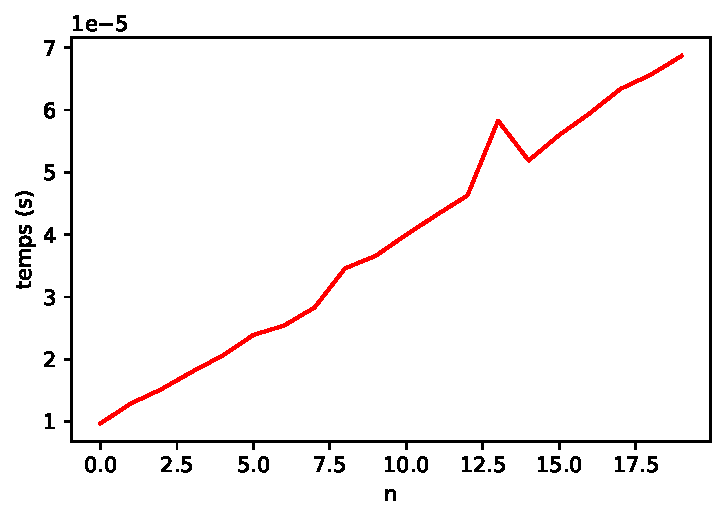
\includegraphics{generalites_files/figure-pdf/cell-2-output-1.pdf}

}

\end{figure}

La courbe obtenue est proche d'une droite, ce qui est cohérent avec la
complexité linéaire de l'algorithme..



\end{document}
